\documentclass[../main.tex]{subfiles}

\graphicspath{{../figures/}}
\usepackage[linesnumbered,ruled,vlined,resetcount,algochapter]{algorithm2e}

\begin{document}

\mychapter{面向大语言模型参数融合的知识引导多形式优化}

% \mysection{符号与缩略语表}{符号与缩略语表}
% \begin{table}
% 	\centering
% 	\caption{}
% 	\small\begin{tabularx}{0.9\textwidth}{ll}
% 		\toprule
% 		\textbf{符号}                                          & \textbf{含义}                                                   \\
% 		\midrule
% 		$\mathcal{M}=\{M_{1},\ldots,M_{n}\}$                 & 专家模型集合(经监督微调的 $n$ 个大模型)                                       \\
% 		$M_{i}$                                              & 第 $i$ 个专家模型                                                   \\
% 		$\mathcal{T}=\{\tau_{1},\ldots,\tau_{k}\}$           & 任务集合(评估所需的 $k$ 个任务)                                           \\
% 		$\tau_{j}$                                           & 第 $j$ 个任务(任务节点)                                               \\
% 		$\mathrm{Merge}(\mathcal{M},\boldsymbol{\alpha})$    & 模型融合算子,以权重 $\boldsymbol{\alpha}$ 合并模型参数                       \\
% 		$\boldsymbol{\alpha}=(\alpha_{1},\ldots,\alpha_{n})$ & 模型融合系数向量                                                      \\
% 		$\mathcal{F}$                                        & 评估函数,用于汇总融合模型的任务表现                                            \\
% 		$w_{j}$                                              & 任务 $\tau_{j}$ 在评估函数中的权重                                       \\
% 		$\mathcal{C}$                                        & 融合系数的约束空间(如单纯形约束$\Delta^{n-1}$)                               \\
% 		$f=(\mathcal{M}_f,\mathcal{T}_f)$                    & 形式(Form),包含一组模型和一组任务的子问题                                    \\
% 		$\ell$                                               & 形式的课程难度级别($\ell$ 通常等于 $\mathcal{M}_f$ 中模型个数)                  \\
% 		$G=(V,E)$                                            & 知识图谱(节点集 $V$ 和边集 $E$ 表示模型与任务关系)                               \\
% 		$s_{ii'}$                                            & 模型 $M_i$ 与 $M_{i'}$ 间的协同分数(知识图谱模型--模型边权重)                     \\
% 		$u_{ii'}$                                            & 模型 $M_i$ 与 $M_{i'}$ 间的关联不确定度                                  \\
% 		$n_{ii'}$                                            & 模型对 $(M_i,M_{i'})$ 被共同观测到的次数                                  \\
% 		$\pi_{ij}$                                           & 模型 $M_i$ 在任务 $\tau_j$ 上的性能统计量(如验证集成绩的滑动平均)                    \\
% 		$\hat{y}_f$                                          & 图神经网络预测的形式 $f$ 的性能评分                                          \\
% 		$\hat{\boldsymbol{\alpha}}_f$                        & 图神经网络预测的形式 $f$ 的模型融合系数                                        \\
% 		$\hat{S}_f$                                          & 图神经网络预测的形式 $f$ 内模型间协同矩阵                                       \\
% 		$\boldsymbol{\alpha}^\star_f$                        & 形式 $f$ 经优化得到的最优融合系数                                           \\
% 		$g_f(i,i')$                                          & 形式 $f$ 中模型 $M_i$ 与 $M_{i'}$ 的协同增益量                            \\
% 		$R$                                                  & 由预测协同矩阵导出的相关矩阵                                                \\
% 		$\sigma(f)$                                          & 形式 $f$ 的不确定性聚合值                                               \\
% 		$\beta_b$                                            & 第 $b$ 次迭代时的探索权重因子                                             \\
% 		\midrule
% 		\textbf{缩略语}                                         & \textbf{含义}                                                   \\
% 		\midrule
% 		LLM                                                  & 大型语言模型                                  \\
% 		SFT                                                  & 监督微调                                  \\
% 		MFTO                                                 & 多形式迁移优化                     \\
% 		KG                                                   & 知识图谱                                         \\
% 		CMA-ES                                               & 协方差矩阵自适应进化策略 \\
% 		GNN                                                  & 图神经网络                                   \\
% 		GAT                                                  & 图注意力网络                               \\
% 		UCB                                                  & 上置信界                                  \\
% 		PRR                                                  & 性能保留率                             \\
% 		M1--M7                                               & 专家模型1--7(对应7个不同领域的微调LLM)                                      \\
% 		\bottomrule
% 	\end{tabularx}
% \end{table}

\mysection{引言}

在上一章对模型结构层的优化方法进行探讨的基础上,本章将研究重点转向参数层的模型融合问题。如今,大型预训练语言模型在各专门领域经过监督微调(Supervised Fine-Tuning, SFT)后,可以获得各具特长的能力。如何在无需额外训练的前提下,将多个此类专长模型的能力集成到一个统一的高性能模型中,成为当前人工智能研究中引人瞩目又极具挑战性的问题。传统的能力增强范式,例如对整个模型进行再次微调,或将多任务数据混合后联合训练单一模型,在当前规模的基础模型上往往计算代价高昂且难以实现。此外,在许多实际场景中,模型可能仅通过黑箱接口提供而无法直接访问参数,这进一步凸显了开发高效的免训练模型融合方法的迫切需求。一个鲁棒的免训练融合策略将使研究者能够模块化地重用已有模型在不同领域和任务上的知识,实现模型能力的按需组装。然而,每个LLM通常包含数十亿参数,并蕴含各自独特且复杂的知识,将它们最优地整合为一对参数配置的搜索无疑是一个极其复杂的优化问题。最简单的融合技术如直接进行参数加权平均等静态启发式方法通常无法获得理想效果,因为不同模型的参数更新可能存在潜在冲突,简单混合同样会导致部分能力的丢失。

早期针对上述难题的研究主要集中于静态的免训练融合算法。例如,Task Arithmetic方法将模型视作基础模型加上任务微调增量的组合,尝试通过对这些任务向量进行算术运算来合成模型;又如 Wortsman 等人的 Model Soup 方案通过对多个微调后模型权重直接求平均,有时能在不增加推理成本的情况下提升性能。这类线性组合尽管简便,在实际中却难以保障融合后模型保留所有任务技能——任意的权重平均往往因参数干扰导致性能退化。为缓解这一问题,后续一些研究提出了更精细的融合策略,例如 SLERP 方法利用球面线性插值来平滑地结合两个模型参数,较直接线性插值产生更平稳的过渡;再如任务向量方法将模型差异表示为对基础模型的参数增量,通过在参数空间中相加减这些增量,可以在不显式训练的情况下实现多任务能力的叠加或移除,相当于对各微调过程的参数变换进行算术级联。这些任务算术思想把模型融合视为对各模型微调参数变换的组合。然而,上述方法大多基于固定的组合规则,而非针对具体问题自适应地优化融合策略,因此在复杂场景下效果有限。

近年来,研究者开始探索优化驱动的模型融合方法,将融合过程视为一个以性能指标为目标的搜索问题,而非预设规则的叠加。例如,模型检查点集成利用贝叶斯优化等技术搜索两个模型按层融合的最佳加权系数;Yadav 等人提出的 TIES-Merging 方法通过在融合前对模型权重进行选择性裁剪和符号对齐,减轻不同模型更新之间的冲突,从而提高直接融合的效果;另一些工作利用训练时统计信息指导无训练的模型域适配,如通过对批归一化参数的调整来在无需微调的情况下适配模型至多个新域。在大语言模型领域,也出现了实用工具(如 MergeKit)实现各类融合算法,表明在实践中组合不同专长的LLM具有实际需求。此外,进化算法也被引入这一问题:有工作尝试用遗传算法高效搜索多模型融合的参数空间,取得了一定效果。总的来看,这些研究确认了模型融合可以被形式化为一个优化问题;但已有方法大多将融合过程视作单阶段完成,即直接试图找到一组全局融合参数(例如针对每层的融合比例)。与此不同的是,本文提出将融合划分为多个阶段递进完成——通过一系列子问题逐步构建最终融合,这在现有模型组合研究中尚属首创。

上述方法主要在模型数量较少、任务维度较低的设定下研究。当待融合模型的数目和任务规模都不大且相当时,搜索空间相对可控,简单的融合方案尚可奏效。然而在现实应用中,可用的已微调专家模型数量往往远超评测任务的数量。实际场景呈现出模型数量远大于任务数量的不平衡局面:常用评测任务集相对稳定且规模有限,而领域专家模型则在不断产生。同一任务可能对应数十个表现各异、部分能力重叠又各有侧重的模型。此时,融合的难点不在于缺少模型技能,而在于如何高效地筛选、加权并整合大量模型。已有为小规模情形设计的方法难以直接扩展到这种大规模不平衡设定,尤其当它们每次融合都从冷启动开始、未能利用相关问题的解来指导当前搜索时,算法将陷入指数级扩张的组合空间。由此可见,有必要引入一种更有原则的框架,将全局融合问题系统性地分解,通过求解较小且 tractable 的子问题提取关系知识,并将其用于指导整体的优化过程。

为此,本章将模型融合问题置于多形式迁移优化(Multi-Form Transfer Optimization, MFTO)的范式下重新审视。MFTO 方法论旨在将复杂优化任务分解为一组更简单的辅助问题(称为形式),这些形式可视作对原问题的不同局部近似或约束版本,并允许在彼此之间共享解和知识。本章中,我们将免训练的大模型融合视为MFTO问题:与其尝试一步到位地求解全局融合,不如设计一系列逐步升级的融合子任务,每个子任务涉及模型或任务的一个子集,或施加了特定约束,使其更易于求解。通过逐一解决这些子问题,我们可以在受控环境下探查模型之间的局部协同或冲突模式,并将这些中间解和关系知识转移回来,指导全局融合的优化。

基于这一思路,我们提出了框架KG-MFTO,即知识引导的多形式优化系统,用于免训练的大模型融合。KG-MFTO包含三个核心模块:(1) 一个动态演化的知识图谱,用图结构显式编码模型–模型和模型–任务间的关系信息;(2) 一个课程规划器,基于知识图谱自适应地序列化各融合子问题(形式),按信息增益最大化的顺序安排求解;(3) 一个知识引导的进化求解器,融合了领域知识以热启动CMA-ES进化算法,用来自知识图谱的先验指导搜索。通过这三者的配合,KG-MFTO实现了优化过程中的持续知识积累与迁移:每当求解一个子问题后,系统都会将所得解及评估结果更新进知识图谱,提炼出模型协作或冲突的模式,再由课程规划器选择下一个最有价值的子问题,并由求解器利用已有知识高效搜索其最优融合配置。如此循环往复,整个融合过程形成一个“感知–计划–行动–学习”的闭环,在完全基于模型推理评价(无梯度)的条件下,实现对大规模模型融合问题的高效求解。

本章的主要贡献如下:首先,我们首次将大模型融合问题形式化为一个多形式迁移优化任务,避免了直接在高维参数空间进行暴力搜索;其次,我们设计并实现了以知识图谱为中心的KG-MFTO系统架构,用结构化记忆来显式表示和传递各形式之间的知识;再次,我们提出了一种课程引导的黑盒搜索策略:由课程规划器动态安排子问题序列构成优化课程,结合基于知识热启动的CMA-ES求解器,实现高效收敛;最后,通过大规模基准实验,我们验证了KG-MFTO在无需训练的情况下成功融合了多个LLM,在多个任务上性能可达到乃至超过各单一模型,并且融合效率显著优于现有方法。消融实验进一步证实了知识图谱、课程规划和双重热启动求解器三者的互补作用。通过对关系知识的显式建模与跨子问题迁移,KG-MFTO为实现可扩展的免训练模型融合提供了一种有原则且高效的途径。我们认为,这一方法为机器学习中的复杂模型复用与组合问题开辟了新的视角。

本章余下内容组织如下:相关工作节介绍与本章研究相关的工作,包括模型无训练融合、任务分解与课程学习、迁移优化以及进化搜索等方面的进展;问题定义与多形式划分节形式化定义了模型融合问题并给出了多形式分解的思路;知识图谱驱动的理论框架节阐述了KG-MFTO的理论框架,包括知识图谱建模和图神经网络推理模块;KG-MFTO算法设计节详细描述了KG-MFTO的算法实现,包括课程规划、知识引导的进化求解器以及整体优化流程;实验与结果分析节给出了实验设置、结果与分析;最后,本章小结节对本章工作进行小结,并说明其与下一章的衔接。

\mysection{问题背景与基础知识}

\mysubsection{模型融合与组合}
在无需额外训练的条件下融合多个已训练模型能力的研究近年来受到关注。一种朴素做法是对模型参数直接进行算术操作:例如 Wortsman 等人提出的模型汤方法表明,对多个微调模型的权重取简单平均有时可提升精度且不增加推理开销。然而,任意的线性加权并不保证保留所有模型的技能,不少情况下简单平均会导致性能下降,这被认为是不同模型参数更新之间的干扰所致。为提高融合稳健性,后续研究探索了多种改进的静态融合策略。例如,球面线性插值通过在高维参数空间沿球面曲线插值两个模型,较线性插值产生更平滑的过渡,从而减小冲突风险;任务向量算术方法将每个模型微调过程视为对基础模型参数的某种移动,提取其参数差分向量,然后通过在参数差分上进行加减,可以在不损害原有性能的情况下实现多任务知识的合成或消除。这种方法在一定程度上保留了各模型对基础模型的增量贡献,但对于参数冲突依然缺乏解决机制。

除了封闭形式的静态融合,也有研究将融合视为需要优化的决策。优化驱动的模型融合方法往往定义一个目标函数(例如在验证数据上的性能),然后搜索使目标最大化的融合配置。例如,Checkpoint Ensembling 方法通过优化确定在逐层参数平均时每个模型的加权系数,使融合后的模型在验证集上性能最佳。Yadav 等人提出的 TIES-Merging 则侧重于在融合前预处理模型参数以减少冲突:他们通过剪除差异较大的权重和对齐参数更新的符号,来缓解直接融合时的互斥效应,再以加权平均完成融合。Yu 等人提出的 DARE 方法受Dropout思想启发,对每个模型的参数增量随机稀疏化后再平均,从而提升融合模型的鲁棒性。还有一些工作尝试利用额外的数据或知识来引导融合,例如无训练的领域自适应:通过对模型的批归一化统计量进行调整,实现模型对新域的适应并与其他模型融合。在大型语言模型的实际应用方面,工具包如 MergeKit 实现了多种融合算法,表明将专门微调的LLM组合起来满足多样任务需求具有实用价值。此外,也有研究将进化算法应用于融合配置搜索:如某进化模型融合方法采用遗传算法在多个模型的融合权重空间中进行搜索,在较少评估次数下找到性能较优的融合方案。总体而言,上述工作将模型融合问题形式化为一个待优化的黑盒搜索任务,并证实了在不进行梯度训练的情况下模型能力的结合是可行的。然而,它们大多只侧重于一次性地求解一个固定规模的融合问题,即直接试图找到同时融合所有候选模型的参数配置。当模型数量和参数维度进一步增大时,这种单阶段暴力搜索变得异常困难。相比之下,我们的方法引入了“多阶段逐步融合”的新思想:通过构造一系列相关的子问题逐步逼近最终融合解,避免直接在全局高维空间中搜索,从而更有效地解决大规模模型融合挑战。

\mysubsection{任务分解与课程式优化}
将复杂任务分解并循序渐进求解的思想在机器学习中由来已久,即所谓课程学习。Bengio 等人在经典工作中表明,以从易到难的顺序呈现训练样本或任务,比起无序混合训练可以使模型收敛更快且泛化更好。虽然课程学习最常用于模型训练情景,其逐步加难的基本原则同样适用于一般优化问题。我们的课程规划器正是借鉴了这一思想:先解决简单的子任务,再逐渐增加难度直至原始问题。在优化领域,这类似于分块坐标迭代等分而治之策略:通过交替优化部分变量、冻结其他变量,使高维问题分解为一系列低维问题来求解。然而,与简单的坐标下降不同,我们的方法并非固定地循环优化各变量块,而是将每个子问题单独近似求解到较优解,并将这些部分解作为构件用于更复杂子问题的初始解或参考。某种意义上,我们的方法也体现了分层与模块化学习的思想:在多任务学习中,研究者有时会先训练若干子模型各自擅长不同任务,然后再将它们集成,这类似于我们首先求解小规模的模型子集或任务子集融合,再通过知识图谱将它们有机结合。通过显式地利用知识图谱记录各子解之间的联系,我们的方法确保了子问题解最终能够一致地整合,而不是简单地各自求解却缺乏整合机制。

一个形象的类比是模型汤的贪心融合过程:在该方法中,多个模型按照效果从高到低依次加入当前汤中,只有当加入下一个模型不会使验证性能下降时才将其纳入融合。这个过程实际形成了一个基于模型的手工课程:每次只融合当前最有价值的一个模型。我们的工作可以看作对此概念的泛化:我们不局限于每次加入单一模型,而是定义了丰富的子问题形式(例如“将模型A与B在任务X上融合”可以算作一种形式),并通过知识图谱和课程规划器自动地从大量候选中选择下一步要解决的融合子任务。这样的顺序并非预先固定的贪心,而是基于当前已经获取的知识由算法自适应决定,体现了一种自动课程学习的思想:序列的决定取决于学习者(这里对应我们的求解器和知识图谱)的状态和进展。在我们的方法中,学习者的状态反映在知识图谱的内容上,而课程规划策略则利用这些知识(例如哪些模型组合尚不确定、哪些子问题的解对全局最有帮助)来选择下一个子任务。由此,任务分解和课程优化在我们的融合问题求解中紧密结合,通过反馈环路实现:早期简单子任务的结果主动影响后续复杂子任务的选择和求解。

\mysubsection{迁移优化与多形式方法}
本章工作深植于进化计算领域的迁移优化(Transfer Optimization, TO)思想。迁移优化旨在利用已解决的相关优化任务的经验来加速新任务的求解,其策略包括顺序迁移和多任务并行优化等。多任务优化允许算法在同一种群中同时进化多个任务的解,个体可以在不同任务之间迁移从而实现知识共享;而多形式迁移优化是近年来提出的一种框架,针对同一个问题的不同形式进行协同优化。所谓形式,是指对同一优化问题的某种变形或子问题,例如低保真度近似、约束松弛版本或子空间子问题等。在MFTO中,研究者人为构造出若干这样的形式,并行或交替地进行优化,同时在这些形式之间交换信息。已有工作多集中在工程设计与多保真度优化领域,例如,用昂贵的高精度目标和廉价的低精度近似目标构成多形式,通过在低精度目标上获取初步解来指导高精度目标的搜索;又如,将单目标问题暂时拓展为多目标问题求解以跳出局部最优,然后再收敛回单目标解(所谓多目标化技术)。在这些例子中,不同形式(高/低保真,单/多目标)共同构成了MFTO框架,算法通过共享种群或定期迁移个体,在形式之间传递有用的部分解和搜索经验。我们的模型融合方法可以被视为MFTO在深度学习模型参数空间中的一次新颖应用:我们设计的每个融合子问题(形式)都是原始融合任务的一个受限版本,可能限定了候选模型子集或任务子集,或降低了优化维度。通过在一系列形式上进行优化,我们得以将原问题的搜索难度拆解,并在形式之间通过知识图谱这一共享记忆池实现知识迁移。值得注意的是,我们采用了图结构来跟踪和指导跨形式的知识转移,这与以往MFTO实现多采用隐式迁移(如共享种群个体)有所不同。通过知识图谱,我们能够表达更加复杂的关系——例如“形式A(模型1+2融合于任务X)的解对于形式B(模型1+2+3融合于任务X)或形式C(模型1+2融合于任务Y)是相关的”,并据此有针对性地将形式A的解用作形式B或C的初始猜测。这种显式的知识跟踪与利用机制提升了迁移优化的效率。

需要强调的是,我们的方法与元学习有本质区别。广义的元学习同样是利用以往任务经验来加速新任务学习,但其典型框架(如MAML)假定任务来自某一分布,目标是学习一个对该分布中任意新任务都能快速适应的模型或初始化。相比之下,我们并不关心将来新的任务,也没有一个独立的“元训练、元测试”阶段——我们所解决的是一个固定的目标问题:融合特定集合的模型来应对特定集合的任务。我们利用多种形式的划分只是为了更高效地解决这一单一问题,而不追求学习一个对其他问题通用的策略。因此,本章的方法严格来说不属于元学习,而是一次性优化过程中的内部迁移和课程机制。这一点有助于明确我们工作的定位:创新点在于如何将复杂融合问题分解并在其内部实现知识迁移,而非训练一个能推广到全新问题的元模型。换言之,KG-MFTO解决的是一个定制的优化实例(虽然内部结构复杂),并不是一个跨任务的学习者。这一区别凸显了我们工作的独特视角:通过对复杂问题内部结构的挖掘和利用,而非跨任务的经验泛化,来加速优化过程。

\mysubsection{知识引导的进化搜索}
最后,我们的方法与进化算法在高维黑盒优化中的应用密切相关。进化算法和遗传算法因其不依赖梯度、易于全局搜索的特点,在优化神经网络权重和结构(即神经进化)方面有悠久历史。近年来,EA被成功应用于神经结构搜索、超参数寻优,甚至直接用于大型模型权重优化等问题。例如,Real 等人(2019)证明了进化策略能够有效发现卷积网络结构,其效果可与梯度驱动的NAS媲美。这说明在复杂离散设计空间中,智能的随机搜索具有强大潜力。在模型融合任务中,前文提到已有尝试利用遗传算法搜索融合系数配置。我们的求解器同样采用了进化式的搜索,但有两点关键区别:一是融入了知识引导,二是细粒度多次搜索而非一次性全局搜索。首先,我们通过知识图谱这一载体,将领域知识注入进化过程。这类似于记忆型算法或带启发的EA:在标准进化操作之外,引入特定领域的启发式以增强搜索效率。常见的方法包括辅助模型的引入,用代理模型预测适应度从而聚焦搜索。在类比下,我们的知识图谱和图神经网络可被视为搜索空间的经验模型,能够提示哪些组合更可能有效。具体而言,我们利用知识图谱预测的解作为种群初始个体,并在变异/交叉时参考已知的优质部分解,从而使搜索不再盲目。其次,与以往对融合问题进行单次全局EA不同,我们在多个形式上运行较小规模的EA,并通过知识图谱使它们协同。这有点类似协同进化的思想:将整体解拆分为若干子部分,各自进化,并定期组合评估整体适应度。在协同进化中,不同子种群优化不同部分变量,然后通过组合形成完整解评估。而我们的形式优化可以看作动态的协同进化:每个形式的进化搜索解决解的一个方面(例如部分模型的权重配置),知识图谱则起到协调作用,确保这些部分最终汇集成一致的全局解。值得注意的是,近期有多任务进化研究开始利用图结构分析任务间的转移关系,这与我们构建图谱规划优化过程的做法不谋而合。通过引入图结构的全局记忆,我们实现了高度分布式却协调一致的搜索:多个进化进程在不同形式上并行展开,但通过知识图谱共享信息并共同收敛到统一的融合模型。

综合来看,我们的方法融合了模型融合领域、迁移优化领域和进化搜索领域的思想创新。我们将模型融合重新定型为MFTO问题,并引入知识驱动的机制(知识图谱与课程规划)来实现形式级别的知识迁移与共享,显著提升了搜索效率。在以下内容中,我们将详细介绍KG-MFTO的方法论,包括如何构建知识图谱表示和课程式的优化过程,以及各模块的实现细节。随后,我们将在实验中验证本章方法在融合多个LLM方面的有效性,并通过与各类基线的比较突出我们方法的优势。

\mysection{问题定义与多形式划分}

首先,我们形式化模型融合问题,并引出多形式分解的求解思路。设有一组已微调的专家模型$\mathcal{M}=\{M_{1}, M_{2}, \ldots, M_{n}\}$,以及一组评估任务$\mathcal{T}=\{\tau_{1}, \tau_{2}, \ldots, \tau_{k}\}$(每个任务均有验证/测试数据)。我们定义一个免训练的融合算子$\mathrm{Merge}(\mathcal{M}, \boldsymbol{\alpha})$,它接受模型集合$\mathcal{M}$及相应融合系数向量$\boldsymbol{\alpha}\in \mathbb{R}^n$,输出融合后的模型参数。同时定义评价函数$\mathcal{F}$来度量融合模型在任务集$\mathcal{T}$上的综合性能。通常,$\mathcal{F}$可表示为各任务指标的加权和,如公式所示:
\begin{equation}
	\begin{aligned}
		\boldsymbol{\alpha}^{\star} & = \arg\max_{\boldsymbol{\alpha}\in\mathcal{C}} \mathcal{F}\Big(\mathrm{Merge}(\mathcal{M},\boldsymbol{\alpha}), \mathcal{T}\Big)                 \\
		{}                          & = \arg\max_{\boldsymbol{\alpha}\in\mathcal{C}} \sum_{j=1}^{k} w_j \text{Score}\Big(\mathrm{Merge}(\mathcal{M},\boldsymbol{\alpha}), \tau_j\Big),
	\end{aligned}
\end{equation}
其中,$\text{Score}(\cdot,\tau_j)$表示融合模型在任务$\tau_j$上的性能度量(如准确率、得分等),$w_j \ge 0$为对应的任务权重且$\sum_{j}w_j=1$,$\mathcal{C}$表示融合系数$\boldsymbol{\alpha}$需满足的约束空间(例如各系数非负且和为1的$n-1$维单纯形$\Delta^{n-1}$)。公式刻画了模型融合的目标:在不给定任何额外训练数据的情况下,通过调整融合权重$\boldsymbol{\alpha}$,使得合并模型在多任务验证集上的加权表现最优。

直接优化高维的$\boldsymbol{\alpha}$以满足目标是非常困难的。当模型数$n$和任务数$k$增大时,搜索空间呈指数级增长,并且不同模型在不同任务上的协同或冲突关系错综复杂,很难通过一次优化找到全局最优的融合配置。为应对这一挑战,本章引入了形式(Form)的概念,将全局融合问题分解为一系列子问题。每个形式 $f=(\mathcal{M}_f,\mathcal{T}_f)$ 由一个模型子集$\mathcal{M}_f \subseteq \mathcal{M}$和一个任务子集$\mathcal{T}_f \subseteq \mathcal{T}$组成,对应求解“仅融合 $\mathcal{M}_f$ 中的模型并在 $\mathcal{T}_f$ 上优化性能”的子任务。显然,全局问题本身也是一种形式,在理想情况下通过若干子形式的求解我们期望逐步逼近全局问题的最佳解。

为此,我们设定了一系列课程难度级别$\ell=2,3,\ldots,L$,其中$\ell$通常对应形式所包含的模型个数(亦即 $|\mathcal{M}_f|=\ell$)。课程学习理念在此体现为:从低级别(如$\ell=2$的简单模型对融合)开始,逐步提升$\ell$合并更多模型,从而增加问题难度。级别$\ell$的所有模型组合形式构成候选集合,在同级别的形式充分探索之后,再进入下一级别。当$\ell$增加时,问题规模越来越接近原始融合任务。通过这样的课程式子问题序列,我们将复杂的全局优化逐步分解为一系列易于求解的小型优化问题。更重要的是,不同形式之间并非相互孤立——通过在较低级别形式中探索获得的部分解和关系知识,我们可以指导更高一级别形式的搜索。例如,在 $\ell=2$ 级别我们或许发现模型 $M_a$ 与 $M_b$ 在某任务上协同效果较好,这一知识在 $\ell=3$ 级别包含 $M_a, M_b$ 的形式中依然有用;又或者我们发现在一个任务子集上某模型权重应被抑制,这可能对包含更多任务的形式也有启发。要充分利用这种跨形式的知识转移,我们需要一种机制来记录和提炼各形式的解之间的关联。本章下一节将介绍我们设计的动态知识图谱,用于作为中心枢纽在优化过程中累积和传播知识,从而将各子问题的解串联成一条完整的推理链,最终服务于全局融合目标的实现。

\mysection{知识图谱驱动的理论框架}

在本节中,我们描述KG-MFTO的理论支撑框架,包括用于跨形式知识共享的知识图谱表示和对图谱进行关系推理的图神经网络模型。知识图谱提供了一个全局视角来整合各子问题的信息,而图神经网络则学习图谱中的关系以预测新子问题的潜在结果和最佳解,从而为课程规划和求解提供指导。

\mysubsection{动态异构知识图谱建模}

我们构建了一个动态异构图 $G=(V,E)$ 来表示模型融合问题中的多种关系。图谱包含两类节点$V=\{\textsc{Model}, \textsc{Task}\}$,以及两类边$E=\{\textsc{Model--Model}, \textsc{Model--Task}\}$,分别对应模型之间的关系和模型与任务之间的关系。

节点表示:每个模型节点$M_i$(对应专家模型$M_i$)被赋予一个可训练的$d$维嵌入表示$\mathbf{h}^M_i \in \mathbb{R}^d$(初始随机化,在优化过程中更新);每个任务节点$\tau_j$ 则使用一个固定的语义向量$\mathbf{h}^T_j \in \mathbb{R}^{d_T}$,该向量可通过预训练的句向量编码器(例如 SimCSE)从任务描述文本或名称计算得到。

边关系及统计量:知识图谱的边刻画了模型间以及模型与任务间的性能关联信息,并随优化过程动态更新。具体而言:

* 每条模型--模型边 $e(M_i, M_{i'})$ 维护两个实值统计量:协同分数 $s_{ii'}$ 和不确定度 $u_{ii'}$。直观地,$s_{ii'}$ 表示模型 $M_i$ 与 $M_{i'}$ 在当前已观察到的融合情形下的合作效果:若 $s_{ii'}$ 为正,表示两模型趋向于互补增益,为负则表示二者存在冲突互斥;$u_{ii'}$ 则表示当前关于 $s_{ii'}$ 的信息不确定程度,反映了我们对该对模型关系的了解充分与否。

* 每条模型--任务边 $e(M_i, \tau_j)$ 记录模型 $M_i$ 在任务 $\tau_j$ 上的性能指标 $\pi_{ij}$(例如验证集精度的指数滑动平均),以及可选的不确定性度量$\upsilon_{ij}$(例如性能的方差估计)。这些数据提供了每个模型在各任务上的擅长程度和稳定性。

知识图谱的边上统计量会在每次完成一个形式的评估后进行更新。假设当前求解了形式 $f=(\mathcal{M}_f,\mathcal{T}_f)$,得到融合配比$\boldsymbol{\alpha}_f$和该融合模型的验证集性能$y_f=\mathcal{F}(\mathrm{Merge}(\mathcal{M}_f,\boldsymbol{\alpha}_f), \mathcal{T}_f)$。我们据此更新图谱边上的统计量:首先,对于任意在 $\mathcal{M}_f$ 中共同出现的模型对 $(M_i, M_{i'})$,计算它们在该形式下的协同增益:
\begin{equation}
	g_f(i,i') = \Big(y_f - \bar{y}^{\text{ref}}_f\Big) \cdot \psi(\alpha_{f,i}, \alpha_{f,i'}),
\end{equation}
其中 $\bar{y}^{\text{ref}}_f$ 是一个参考基准得分,用于衡量本次融合结果相对于基线的提升程度(例如 $\bar{y}^{\text{ref}}_f$ 可取 $\mathcal{M}_f$ 中单个最好模型在 $\mathcal{T}_f$ 上的得分或所有模型简单平均融合的得分);$\psi(\alpha_{f,i},\alpha_{f,i'})$ 则是一个用于度量模型 $M_i$ 与 $M_{i'}$ 共同贡献的函数,取值范围限定在$(-1,1)$。在简单情况下,可取 $\psi(a,b)=2ab$(当 $\boldsymbol{\alpha}$ 属于概率Simplex时,这表示两模型权重都较大时协同效应更强)。有了$g_f(i,i')$,我们采用滑动平均来更新协同分数:
\begin{equation}
	s_{ii'} \leftarrow (1-\lambda) s_{ii'} + \lambda g_f(i,i'),
\end{equation}
其中 $0<\lambda\ll 1$ 为平滑系数。通过持续积累不同形式中的协作增益$g_f(i,i')$,$s_{ii'}$ 将逐渐收敛到模型对 $(i,i')$ 在全局融合中的实际交互关系:若二者经常在一起出现在高性能融合解中,$s_{ii'}$ 会变为较大的正值;反之若二者共存时性能往往低于参考,$s_{ii'}$ 将趋向负值。

接下来,我们更新模型对的不确定度 $u_{ii'}$。一种简单的做法是记录该模型对在多少个不同形式中被观测到,然后根据观测次数递减不确定度。例如:
\begin{equation}
	\begin{aligned}
		n_{ii'} & \leftarrow n_{ii'} + \mathbb{I}\{i,i'\in\mathcal{M}_f\}, \\
		u_{ii'} & \leftarrow \frac{\kappa}{\kappa + n_{ii'}},
	\end{aligned}
\end{equation}
其中$\mathbb{I}(\cdot)$为指示函数,$n_{ii'}$ 累计了模型 $i$ 和 $i'$ 被一起包含于形式的次数,$\kappa$是初始虚拟观测次数(例如$\kappa=1$使得初始$u_{ii'}=0.5$)。这样,当某对模型尚未或很少被共同评估时,不确定度接近1;而随着其被考察次数增多,$u_{ii'}$ 单调减小,表示我们对其关系的信心提高。除了这种频次方法,亦可维护协同增益$g_f(i,i')$值的方差估计,将不确定度建模为方差的指数滑动平均$u_{ii'} \leftarrow \rho u_{ii'} + (1-\rho)\hat{\sigma}_{ii'}^2$,但无论采用何种策略,不确定度都会随证据增多而下降。

最后,对于每个参与当前形式的模型 $M_i\in \mathcal{M}_f$ 和任务 $\tau_j \in \mathcal{T}_f$,我们更新模型--任务边的性能指标$\pi_{ij}$,例如通过记录融合模型在任务$\tau_j$上的得分,或者对先前$\pi_{ij}$取加权平均。这一步可以视为对模型 $M_i$ 在任务 $\tau_j$ 上能力的重新校准:如果 $M_i$ 参与的融合在 $\tau_j$ 上取得了好的结果,说明 $M_i$ 对该任务可能有所助益;反之亦然。模型--任务边的不确定度$\upsilon_{ij}$亦可类似更新。

需要强调,知识图谱是随优化过程动态演化的:初始时我们对任何模型关系都不了解,可将所有 $s_{ii'}$ 设为0、$u_{ii'}$ 设为1(最大不确定);随着逐步评估各种形式,图谱记录的信息愈加丰富,所包含的知识也愈加准确。知识图谱在整个融合求解过程中扮演全局记忆库的角色:它显式存储了各模型之间、模型与任务之间已经探明的关系,为后续未探明的组合提供指导依据。

\mysubsection{图神经网络的关系推理}

有了上述知识图谱表示,我们进一步设计了一个异构图注意力网络来对图谱进行推理,预测未观察过的形式的性质。该GNN从图谱中提取与某候选形式$f=(\mathcal{M}_f,\mathcal{T}_f)$相关的子图信息,并输出对该形式的性能、最优融合系数以及模型关系的预测。这为课程规划器选择形式和求解器热启动提供了关键依据。

具体而言,我们采用节点类型特定的线性变换将初始嵌入投影到共同空间:$\tilde{\mathbf{h}}^{M}_i = W_M \mathbf{h}^{M}_i$,$\tilde{\mathbf{h}}^{T}_j = W_T \mathbf{h}^{T}_j$,其中 $W_M \in \mathbb{R}^{d'\times d}$ 和 $W_T \in \mathbb{R}^{d'\times d_T}$。接下来,GNN包含$L$层图注意力网络,每层针对异构边类型分别计算注意力权重。对于模型--模型边,我们将边特征(如 $s_{ii'}$ 和 $u_{ii'}$)融合到注意力计算中,从而使具有高协同分数的模型节点对在消息传递时权重更高,而高不确定度可以暂时赋予其更大注意力以获取新信息;对于模型--任务边,则根据$\pi_{ij}$权重来调整模型节点与任务节点之间的信息流强度。通过这种边权重调制的注意力机制,GNN能够根据知识图谱中已有的关系数据,更加精准地聚合邻居信息。经过 $L$ 层传播后,我们获取了每个节点的高阶表示,记为 $\mathbf{z}^M_i$(模型节点)和 $\mathbf{z}^T_j$(任务节点)。

为了得到针对某一候选形式$f$的预测,我们取出该形式诱导的子图,即包含 $\mathcal{M}_f$ 中的模型节点及 $\mathcal{T}_f$ 中的任务节点,以及它们之间的所有连边。然后,在这个子图上应用三个并行的输出头进行汇聚:

\textbf{(1)性能预测头}:对形式$f$输出一个标量 $\hat{y}_f$,用于预测该形式在综合评价函数$\mathcal{F}$下的得分。这可以通过对子图中的模型节点和任务节点的表示进行某种聚合来实现,例如将所有模型节点表示与任务节点表示拼接后通过多层感知机回归出$\hat{y}_f$。我们希望$\hat{y}_f$尽可能逼近真实的 $y_f$。

\textbf{(2)权重预测头}:输出形式$f$中各模型的融合权重预测$\hat{\boldsymbol{\alpha}}_f = (\hat{\alpha}_{f,i}: M_i \in \mathcal{M}_f)$。由于不同形式的$\mathcal{M}_f$大小各异,我们采用自注意力机制实现对可变长度集的映射:具体地,引入一个轻量级Transformer编码器,令形式中的每个模型节点表示$\mathbf{z}^M_i$作为Transformer的输入序列,经若干注意力层后,输出维度与$\mathcal{M}_f$大小相同,对应预测的每个模型权重$\hat{\alpha}_{f,i}$(通过软max归一化使其和为1)。这样设计可以根据模型节点间的相对关系来分配权重。这个头的作用是直接给出融合配置的建议,供后续求解器参考。

\textbf{(3)协同预测头}:输出形式$f$中各模型对的协同矩阵$\hat{S}_f \in \mathbb{R}^{m\times m}$($m=|\mathcal{M}_f|$)。我们让该头输出对称矩阵,其中 $(\hat{S}_f)_{ii'}$ 反映模型 $M_i$ 与 $M_{i'}$ 在形式$f$下的交互强弱预测。具体实现上,可以让每个模型节点最终表示$\mathbf{z}^M_i$通过一个前馈网络映射到一个$h$维向量,然后定义 $(\hat{S}_f)_{ii'} = \phi(\mathbf{q}_i^\top \mathbf{q}_{i'})$,其中$\mathbf{q}_i$为模型$M_i$对应的$h$维向量,$\phi(\cdot)$为一个压缩函数(如双曲正切),以确保输出范围有限。协同预测头旨在提前估计当前形式内部模型两两之间是正协同(互补)还是负协同(冲突)。

图神经网络通过在线学习不断提高上述预测的准确性。每当一个形式$f$被实际评估后,我们将其真实结果 $(y_f, \boldsymbol{\alpha}_f^\star)$ 作为训练样本,对GNN的参数进行更新。训练损失函数设计为同时兼顾三种预测的误差:
\begin{equation}
	\mathcal{L}_{\text{GNN}} =
	w_{\text{perf}}\big(\hat{y}_f - y_f\big)^2
	+
	w_{\alpha}\text{KL}\big(\boldsymbol{\alpha}_f^\star | \hat{\boldsymbol{\alpha}}_f\big)
	+
	w_{\text{syn}}\big|\hat{S}_f - S^{\text{KG}}_f\big|_F^2,
\end{equation}
其中 $w_{\text{perf}}, w_{\alpha}, w_{\text{syn}}$ 为超参数权重;$\text{KL}(\cdot|\cdot)$ 表示两个分布(向量经归一化后)的KL散度,用于度量预测的权重与当前已知最佳权重之间的差异;$|\cdot|_F$ 为Frobenius范数;$S^{\text{KG}}_f$ 为从当前知识图谱中提取的该形式的目标协同矩阵。例如可令 $(S^{\text{KG}}_f)_{ii'} = s_{ii'}$(对于 $i,i'\in \mathcal{M}_f$),即将当前图谱存储的协同分数作为期望值;或者简单地取 $S^{\text{KG}}_f$ 为0矩阵以鼓励 GNN 输出的小幅度。通过最小化损失,GNN 学会用自身的预测逼近知识图谱中的已有知识和当前求解得到的新知识。这里的KL散度项确保 GNN 建议的融合配比逐渐贴近目前观察到的最佳配比,从而提高日后对类似形式的指引作用;而协同矩阵误差项则让 GNN 内隐地学习模型对的相互作用规律。当不断有新形式解入图训练时,GNN 的预测性能会持续提升,进而帮助我们更好地评估和选择尚未探索的形式。换言之,图神经网络在整个优化过程中充当代理模型或导航员的角色:它将知识图谱中零散的关系数据综合为对新问题的预测,为何种组合值得尝试、该如何初始化解提供智能化建议。

通过知识图谱与图神经网络这两部分,我们构建了一个显式建模关系知识并随经验自我改进的理论框架。下一节中,我们将在此基础上介绍KG-MFTO的算法流程,包括如何利用GNN的预测来规划课程、选择形式,以及设计何种求解策略来充分利用这些知识进行融合优化。

\mysection{KG-MFTO算法设计}

本节详细介绍 KG-MFTO 框架下各模块的算法实现,包括课程规划器用于候选形式的生成与选择,知识引导的进化求解器用于高效求解单个形式的最优融合配比,以及二者与知识图谱之间的闭环协作过程。整个算法遵循“感知-计划-执行-学习”的循环,我们将在伪代码和文字解释中展现这一闭环的具体运作。

\mysubsection{课程规划与形式选择}
在每次迭代中,KG-MFTO的课程规划器负责决定下一步要解决的融合子问题(形式)。规划器首先在当前课程级别$\ell$产生一组候选形式,然后利用图神经网络的预测值对这些候选进行评分,选出最优的形式提交给求解器。这样,规划器相当于在形式空间上进行了一步决策搜索,以期每次选择都能带来最大的信息增益和性能提升。

\mysubsubsection{候选形式生成}

给定当前课程级别 $\ell$,我们希望产生若干候选形式,每个形式包含 $\ell$ 个模型。为了高效探索形式空间,我们采用一种混合启发的随机生成策略。在生成每一个候选形式时,我们以一定概率从以下三种策略中选择一种:

\begin{itemize}[leftmargin=3\ccwd]
	\item \textbf{不确定性引导策略}(概率 $p_{\text{unc}}$):随机选取当前知识图谱中不确定度最高的一对模型$(M_i, M_{i'})$,强制令其包含在形式中,然后随机加入其他 $\ell-2$ 个模型补足大小。这样得到的形式至少包含一个尚未充分探索过的模型对,旨在通过评估该形式来消除高不确定区域。
	\item \textbf{协同引导策略}(概率 $p_{\text{syn}}$):先从图谱中选取某个模型$M_i$作为种子,然后基于当前 GNN 预测的协同矩阵 $\hat{S}$,贪婪地选择与$M_i$协同分数$\hat{s}_{ij}$较高的模型逐个加入,直至形成大小为$\ell$的一个强协同集合。直观上,这倾向于构造那些 GNN 已预测为可能有较强正协同效果的模型组合,以验证这些预测并在成功时快速累积性能。
	\item \textbf{随机策略}(概率 $1 - p_{\text{unc}} - p_{\text{syn}}$):在剩余情况下,简单地在所有 $\binom{n}{\ell}$ 种大小为$\ell$的模型子集中均匀随机采样一个形式。这样可以保持探索的多样性,避免陷入仅依据当前预测的贪心选择。
\end{itemize}

此外,无论通过何种策略生成形式$f=(\mathcal{M}_f,\mathcal{T}_f)$,我们还将相应选择一个任务子集$\mathcal{T}_f$。一般而言,我们让$\mathcal{T}_f$尽量包含代表性的任务以全面评估性能,但在某些阶段也可采用聚焦策略,例如固定$\mathcal{T}_f$为导致模型冲突最大的那几个任务,以专门优化那方面性能。为了确保比较的公平性,我们要求 $\mathcal{T}_f$ 至少覆盖全局评价函数$\mathcal{F}$中涉及的主要指标。例如,在我们的实验中,每个$\mathcal{T}_f$都包含四大基准任务中的至少两个,以避免只优化单一任务导致偏离全局目标。

通过上述过程重复生成,直到收集到 $K$ 个候选形式$\mathcal{C}_\ell$($K$为预设候选池大小)。算法展示了候选形式生成的伪代码流程。需要注意的是,$K$ 并不需要很大,因为后续的评分选择将缩小范围;而且我们在生成过程中已经注入了启发式引导,使得这有限的候选中较大概率包含有价值的形式。

\begin{algorithm}[tb]
	\small
	\DontPrintSemicolon
	\KwIn{模型集 $\mathcal{M}$,任务集 $\mathcal{T}$,知识图谱 $G$,当前级别 $\ell$,候选池规模 $K$}
	\KwOut{候选形式集合 $\mathcal{C}_\ell$}
	$\mathcal{C}_\ell \leftarrow \emptyset$;
	\While{$|\mathcal{C}_\ell| < K$}{
		\eIf{\texttt{rand()} $< p_{\text{unc}}$}{
			从图谱中选取当前不确定度最高的模型对 $(M_u, M_{u'})$;\\
			设 $\mathcal{M}_f \leftarrow \{M_u, M_{u'}\}$ ;
		}{\eIf{\texttt{rand()} $< p_{\text{unc}} + p_{\text{syn}}$}{
				从$\mathcal{M}$中随机选取一个模型 $M_s$ 作为种子;\\
				依据当前$\hat{S}$将与 $M_s$ 协同值最高的 $\ell-1$ 个模型加入$\mathcal{M}_f$;
			}{
				从$\mathcal{M}$中均匀随机抽取 $\ell$ 个不同模型组成 $\mathcal{M}_f$;
			}}
		按需要选择 $\mathcal{M}_f$ 上的任务子集 $\mathcal{T}_f \subseteq \mathcal{T}$,确保覆盖主要评估指标;\\
		将 $f=(\mathcal{M}_f,\mathcal{T}_f)$ 加入 $\mathcal{C}_\ell$;
	}
	\Return{$\mathcal{C}_\ell$}
	\caption{候选形式生成 (级别 $\ell$)}
	\label{alg:candidates}
\end{algorithm}

形式评分与选择:一旦得到候选形式集$\mathcal{C}_\ell$,我们利用上一节训练好的 GNN 对每个候选形式 $f\in\mathcal{C}_\ell$ 进行预测,并据此计算一个评分 $A(f)$ 来衡量其价值。我们采用类上置信界的评分策略:
\begin{equation}
	A(f) = \hat{y}_f + \beta_b \sigma(f),
\end{equation}
其中 $\hat{y}_f$ 是 GNN 性能头预测的形式$f$综合得分,$\sigma(f)$ 则是对该形式不确定性的量化。我们将 $\sigma(f)$ 定义为形式$f$中所有模型对边不确定度$\{u_{ii'}: i,i'\in \mathcal{M}_f\}$的某种聚合,如简单平均或截断平均(去除最高和最低若干值后的均值),以代表$f$内部关系知识的未知程度。$\beta_b$ 是一个随着迭代轮次 $b$ 递减的探索系数(例如$\beta_b = \beta_0 / \sqrt{1+b}$),在算法初期保持较大以鼓励探索高不确定区域,后期逐渐减小以更加依赖模型预测的$\hat{y}_f$进行利用。通过UCB评分,如果某形式的预期性能$\hat{y}_f$很高则其评分自然高;同时如果某形式涉及的关系大多尚不明确($\sigma(f)$高),其评分中也会加上一定的探索红利,鼓励算法尝试新组合获取知识。反之,如果形式的几乎所有关系都已有充分认知($\sigma(f)$低),那么除非 $\hat{y}_f$ 非常高,否则规划器会倾向于选择别的形式,以避免重复探索收益有限的区域。可以看出,UCB评分在这里平衡了性能导向和知识获取导向两种考虑。

计算出所有候选的 $A(f)$ 后,课程规划器从 $\mathcal{C}_\ell$ 中选出得分最高的形式$f^\star = \arg\max_{f\in\mathcal{C}_\ell} A(f)$ 作为本次迭代的目标形式。随后,系统将把$f^\star$ 交由融合求解器进行优化。值得一提的是,我们还在规划器中设置了课程级别提升的判定条件:当当前级别$\ell$的形式组合情况已较为充分地覆盖到下一级别$\ell+1$的所有模型对时(例如对于$\ell+1$级别涉及的每对模型,我们在$\ell$级别至少观察过一次),则认为可以适时提升课程级别 $\ell \leftarrow \ell+1$。这样做是为了防止算法在低级别停留过久,从而能及时扩大组合规模,逐步接近全局融合问题。同时,这一条件确保在进入更高难度前,我们已对更小组合的关系有了基本了解,从而减小盲目性。课程级别提升通常与不确定度阈值或观察覆盖率等指标相关,可根据需要灵活设定。

\mysubsection{知识引导的进化求解器}
选定形式$f^\star$后,我们需要在不给定梯度信息的情况下优化公式在该子问题上的目标,即求解:
$\boldsymbol{\alpha}^\star_{f^\star} = \arg\max_{\boldsymbol{\alpha}\in \mathcal{C}_{f^\star}} \mathcal{F}\Big(\mathrm{Merge}(\mathcal{M}_{f^\star}, \boldsymbol{\alpha}), \mathcal{T}_{f^\star}\Big),$
其中 $\mathcal{C}_{f^\star}$ 表示融合算子在形式$f^\star$下的系数约束空间(例如 $\sum_{i\in \mathcal{M}_{f^\star}} \alpha_i = 1$ 且 $\alpha_i \ge 0$)。由于融合目标对 $\boldsymbol{\alpha}$ 来说是黑盒的且高度非凸,我们采用进化策略中的 CMA-ES 算法来执行这一优化搜索。CMA-ES 是一种协方差矩阵自适应的演化算法,在连续参数优化中具有强大的全局搜索能力和鲁棒性。但为了充分利用本章框架中的知识,我们对CMA-ES进行了双重热启动:即通过知识图谱和 GNN 对目标形式的预测结果,初始化 CMA-ES 的搜索分布,使其从一个极具潜力的区域开始搜索,从而大幅减少试探开销。

在具体展开前,我们将融合系数的优化变量$\boldsymbol{\alpha}$进行适当的参数化,使其对无约束演化算法更加友好。
若融合系数要求为概率分布(如简单平均),我们采用Softmax参数化。引入自由参数向量$\mathbf{z}\in \mathbb{R}^m$($m=|\mathcal{M}_{f^\star}|$),通过 $\alpha_i = \frac{\exp(z_i)}{\sum_{i'} \exp(z_{i'})}$ 将其映射到 $\Delta^{m-1}$ 单纯形。这确保无论如何搜索,$\boldsymbol{\alpha}$ 都满足非负和和为1的约束。为避免数值问题,可设定$z_i$的上下界(如$[-10,10]$)防止softmax输出极端0或1。
若融合允许权重取正负(如对参数增量进行叠加的情形),我们采用tanh参数化。$\alpha_i = \frac{\tanh(z_i)}{\sum_{i'}|\tanh(z_{i'})|}$,这样$z_i$ 任意实数均可通过 $\tanh$ 压缩在 $(-1,1)$,再归一化保证和为1的绝对值。直观上,这是对正负贡献进行归一的表示。

有了$\mathbf{z}$的无约束表示,我们便可以在$\mathbb{R}^m$上运行 CMA-ES 了。CMA-ES以正态分布作为演化的候选分布,其核心在于每代更新分布的均值和协方差矩阵,使其逐步收敛到高适应度区域。在初始化时,我们需要给定一个起始均值 $\mathbf{m}_0$ 和一个初始协方差矩阵 $C_0$。这里,我们利用 GNN 预测的输出来设定它们:

\textbf{均值热启动}:将 GNN Alpha Head 输出的$\hat{\boldsymbol{\alpha}}_{f^\star}$作为起点,即令 $\mathbf{m}_0 = \mathcal{R}(\hat{\boldsymbol{\alpha}}_{f^\star})$,其中 $\mathcal{R}(\cdot)$ 表示将融合权重逆映射到$\mathbf{z}$空间的函数。对于softmax参数化,这相当于取 $\mathbf{m}_0$ 的各分量 $m_{0,i} = \log(\hat{\alpha}_{f,i} + \varepsilon)$ 减去平均值($\varepsilon$为一个很小的数,如1e-6,用于避免取对数时零值),以保证对应的$\mathbf{z}$映射回$\hat{\boldsymbol{\alpha}}_{f}$;对于tanh参数化,我们可取 $m_{0,i} = \tanh^{-1}(\hat{\alpha}_{f,i})$(将超出$(-1,1)$范围的预测裁剪到$-0.99,0.99$以计算反双曲正切)。这个初始化使得演化算法一开始就从 GNN 建议的融合配置附近开始搜索。$\hat{\boldsymbol{\alpha}}_{f^\star}$ 本身已经融合了知识图谱和过往形式解的信息,是较优解的预测,因此以其为中心启动搜索能够显著减少探索的盲目性。

\textbf{协方差热启动}:利用 GNN Synergy Head 输出的预测协同矩阵 $\hat{S}_{f^\star}$ 来设定初始协方差的相关结构。我们先将 $\hat{S}_{f^\star}$ 转换为相关矩阵:对于 $i \neq i'$,定义
\begin{equation}
	R_{ii'} = \phi\Big((\hat{S}_{f^\star})_{ii'}\Big),
\end{equation}
其中 $\phi(\cdot) = \tanh(\gamma \cdot)$ 是一个S型函数($\gamma>0$为缩放因子),用于将预测协同值映射到$(-1,1)$内,作为相关系数的近似。$R_{ii}=1$ 对角线元素保持为1。由于 $\hat{S}_{f^\star}$ 可能不是正定矩阵,我们对 $R$ 做特征值分解 $R=Q\Lambda Q^\top$,将所有特征值$\lambda_i$裁剪为非负(如$\max(\lambda_i,\epsilon)$,$\epsilon$取$10^{-6}$),再重构$R$以确保其为半正定矩阵。最后选定一个初始尺度参数 $\sigma_0>0$,设置初始协方差矩阵为 $C_0 = \sigma_0^2 R$。这样产生的初始分布 $\mathcal{N}(\mathbf{m}_0, C_0)$ 具有以下意义:其均值在前述高潜力解附近,同时模型间的初始采样相关性反映了 GNN 预测的模型协同关系。若 $\hat{S}_{f^\star}$ 显示某两个模型高度正相关(可能需要一起取较大权重才能出好效果),则 $R$ 中对应的相关系数为正,使得它们的采样值倾向于同增同减;若协同为负,则产生负相关采样,使得它们的权重一增一减。这一协方差热启动有效地将知识图谱蕴含的模型依赖关系注入到随机搜索中,使CMA-ES更快找到满足协同约束的区域。

完成初始化后,我们运行 CMA-ES 对 $\mathbf{z}$ 进行迭代优化。在每次评价候选 $\mathbf{z}$ 时,我们先通过 $\mathrm{Proj}(\mathbf{z})$ 将其映射成融合系数$\boldsymbol{\alpha}$,然后调用评估函数返回 $\mathcal{F}(\mathrm{Merge}(\mathcal{M}_{f^\star}, \boldsymbol{\alpha}), \mathcal{T}_{f^\star})$。为了减小评估噪声对搜索的影响,我们采用多次前向传播取中值的方式评估模型性能:对每个候选融合模型,我们在验证集上用不同随机种子跑多次前向推理,将这些分数取中位数作为该候选的适应度值(这相当于中值滤波,降低了随机因素或评价不稳定性的干扰)。CMA-ES 将根据这些适应度更新其内部的均值和协方差参数。当发现算法停滞(如连续$G_{\text{stall}}$代没有更优解出现)时,我们触发信赖域重启:将协方差 $C$ 缩小,例如将$\sigma_0$减半后重置$C_0=\sigma_0^2 I$(或 $C$ 的对角线),从当前均值$\mathbf{m}$重新开始局部搜索。这相当于在均值已近优、但协方差未充分收敛时,强行收缩搜索范围以 fine-tune 解。另一方面,如果我们观察到协方差矩阵的条件数急剧增大或者算法出现过早收敛迹象,也可能说明 GNN 提供的先验有误导,此时我们会采取降温措施:例如将 $C$ 与单位矩阵组合 $C \leftarrow (1-\eta)C + \eta \sigma^2 I$ 以降低相关性影响,或完全重置协方差为各维独立(对角矩阵)以重新探索。经过这些机制的增强,CMA-ES 通常能够高效逼近形式$f^\star$的最优融合解。

算法 给出了知识引导求解器对单个形式进行优化的过程概要。最后输出的$\boldsymbol{\alpha}^\star_f$连同相应得分$y_f$将返回给主循环,用于更新知识图谱和训练GNN。

\begin{algorithm}[tb]
	\small
	\DontPrintSemicolon
	\KwIn{形式 $f=(\mathcal{M}_f,\mathcal{T}_f)$,GNN预测 $(\hat{y}_f,\hat{\boldsymbol{\alpha}}_f,\hat{S}_f)$,融合算子 $\mathrm{Merge}$,评价函数 $\mathcal{F}$}
	\KwOut{形式 $f$ 的最优融合方案 $\boldsymbol{\alpha}^\star_f$ 及其得分 $y_f$}
	$(\mathbf{m}_0,C_0)\leftarrow$ \textbf{WarmStart}$\big(\hat{\boldsymbol{\alpha}}_f, \hat{S}_f\big)$
	$\displaystyle \boldsymbol{\alpha}^\star_f \leftarrow \textbf{CMA-ES}\Big(\mathbf{m}_0, C_0, \text{fitness}= \big\{\mathbf{z} \mapsto \mathcal{F}\big(\mathrm{Merge}(\mathcal{M}_f, \mathrm{Proj}(\mathbf{z})), \mathcal{T}_f\big)\big\}\Big)$ ;
	$y_f \leftarrow \mathcal{F}\Big(\mathrm{Merge}(\mathcal{M}_f, \boldsymbol{\alpha}^\star_f), \mathcal{T}_f\Big)$
	\Return{$(\boldsymbol{\alpha}^\star_f,y_f)$}
	\caption{知识引导的融合求解器(单个形式)}
	\label{alg:solver}
\end{algorithm}

\mysubsection{闭环优化与图谱更新}
形式$f^\star$求解完成后,KG-MFTO 进入学习步骤,即根据新获得的成果更新知识图谱和 GNN,从而完成一次闭环。具体步骤如下:首先,我们将形式$f^\star$的解$\boldsymbol{\alpha}^\star_{f^\star}$及其性能$y_{f^\star}$用于更新知识图谱中的边属性:对于$f^\star$中每一对模型$(M_i,M_{i'})$,计算$g_{f^\star}(i,i')=(y_{f^\star}-\bar{y}^{\text{ref}}_{f^\star})\cdot 2\alpha^\star_{f^\star,i}\alpha^\star_{f^\star,i'}$并相应地更新协同分数 $s_{ii'}$ 以及观测次数 $n_{ii'}$ 和不确定度 $u_{ii'}$;同时,对于$f^\star$涉及的每个模型和任务,我们更新模型--任务性能$\pi_{ij}$(例如取之前值与本次融合模型在任务$\tau_j$表现的加权平均)。接着,以$(f^\star,\boldsymbol{\alpha}^\star_{f^\star},y_{f^\star})$作为新的训练样本,对图神经网络执行数步梯度下降以最小化损失,更新 GNN 参数,使其能够重现该形式的结果。通过这一步,知识图谱和代理模型都更为聪明:图谱中显式存储了新的模型关系数据,GNN 则隐式将这些数据泛化为对其它潜在形式的更新预测。

完成学习后,我们检查课程级别是否需要调整:如前所述,若当前级别的形式探索已达到预设充分度且尚未达到最大级别,则令$\ell \leftarrow \ell+1$,以便下次迭代生成更大规模的形式来求解。随后进入下一循环。整个闭环将持续运行直到耗尽预设的评估预算 $B$(即最多评估 $B$ 个形式的性能),或达到其它终止条件(如已找到全局融合的满意解)。最终,知识图谱中应已存有关于各模型关系的丰富知识,而我们也获得了一系列所求解过的形式及其融合方案,其中最高级别(通常即全体模型)的融合方案即为我们想要的最终结果。算法 综合展示了 KG-MFTO 的完整流程。可以看到,课程规划、求解和图谱更新彼此交替,构成了一个自适应的闭环优化算法。

\begin{algorithm}[tb]
	\small
	\DontPrintSemicolon
	\KwIn{模型集 $\mathcal{M}$,任务集 $\mathcal{T}$,融合算子 $\mathrm{Merge}$,评估预算 $B$}
	\KwOut{得到解的形式集合及对应融合方案 $\{(f,\boldsymbol{\alpha}_f^\star,y_f)\}$}
	初始化知识图谱 $G$(节点包括$\mathcal{M}$和$\mathcal{T}$,边协同 $s_{ii'}=0$,不确定度 $u_{ii'}=1$ 等);\ 初始化 GNN 参数(例如将 GNN 输出初始化为无偏估计:$\hat{y}\approx$单模型表现,$\hat{\boldsymbol{\alpha}}\approx$均匀分配,$\hat{S}\approx 0$);\\
	设课程级别 $\ell\leftarrow 2$,已评估形式数 $b\leftarrow 0$;\\
	\While{$b < B$}{
		$\mathcal{C}_\ell \leftarrow \textbf{GenerateCandidates}(\mathcal{M},\mathcal{T},G,\ell,K)$
		\For{\textbf{each} $f \in \mathcal{C}_\ell$}{
			用当前 GNN 预测 $(\hat{y}_f,\hat{\boldsymbol{\alpha}}_f,\hat{S}_f)$;\\
			计算 $\displaystyle \sigma(f) = \text{Agg}\big(\{u_{ii'}: i,i'\in\mathcal{M}_f\}\big)$ (如取平均);\\
			计算 $A(f) = \hat{y}_f + \beta_b\sigma(f)$ ;
		}
		选取 $f^\star = \arg\max_{f\in \mathcal{C}_\ell} A(f)$ 为本次迭代要评估的形式;\\
		$(\boldsymbol{\alpha}_{f^\star}^\star,y_{f^\star})\leftarrow \textbf{SolveForm}\big(f^\star,\hat{\boldsymbol{\alpha}}_{f^\star},\hat{S}_{f^\star},\mathrm{Merge},\mathcal{F}\big)$
		使用 $(f^\star,\boldsymbol{\alpha}_{f^\star}^\star,y_{f^\star})$ 更新知识图谱 $G$和训练 GNN;\\
		令 $b\leftarrow b+1$;
		\If{\textbf{需要提升级别}(依据累积观测覆盖率等)}{
			$\ell \leftarrow \ell + 1$;
		}
	}
	\caption{KG-MFTO:知识引导的多形式迁移优化算法流程}
	\label{alg:kg-mfto}
\end{algorithm}

\mysubsection{实践要点与扩展}
上述KG-MFTO算法框架在实践中可根据需要进行一些调整与扩展,以增强稳定性和适应不同场景:

\textbf{分层融合系数表示}:在某些融合算子中,允许针对模型的不同部分赋予不同权重(例如各 Transformer 层分别融合)。此时直接优化维度会变得极高。我们可以对融合系数使用低秩结构参数化,例如令$\alpha^{(\ell)}_i = \frac{\exp(a_i + b_\ell)}{\sum_{i'} \exp(a_{i'} + b_\ell)}$,将每个模型的整体重要性$ a_i$ 和每一层的偏置 $b_\ell$ 分别设为参数,加上小的交互项以增加表达能力。这样,优化变量从每层每模型一个,减少为每模型一个和每层一个,大幅降低维数。CMA-ES即可以在$\{a_i\}$和$\{b_\ell\}$空间运行。通过这种方式,本章方法可拓展用于逐层(或模块)融合的情形,并通过知识图谱学习层级之间的模式。

\textbf{任务权重调整}:在多任务融合中,不同任务的评价尺度和可靠性可能差异较大。为防止某些任务主导优化或被忽略,我们可以对$\mathcal{F}$的任务加权$w_j$进行动态调整。例如,根据各任务得分的方差或不确定性设定$w_j \propto 1/\widehat{\mathrm{Var}}(\text{Score}(\cdot,\tau_j))$,使评价更稳定;或在求和前对各任务分数进行排序归一化,以减小尺度差异带来的影响。这些技术有助于提升融合结果的任务公平性和稳健性。知识图谱中模型--任务边的性能不确定度$\upsilon_{ij}$也可以用来辅助调整$w_j$。

\textbf{冷启动与校准}:在优化开始时,由于没有任何形式评估数据,GNN预测可能完全没有依据。我们通过对单模型行为的自监督预训练来初始化GNN:令性能头预测$\hat{y}_f$逼近选用单一模型时各任务的得分之和,Alpha头输出接近“给予表现最佳的单模型以全部权重”,Synergy头输出趋近0矩阵。这相当于告诉 GNN:在没有知识时,倾向于认为只有一个模型起主要作用,模型间既无特别协同也无特别冲突。这样初始化可避免 GNN 输出的无意义值误导初期搜索。此外,在 GNN 训练中我们采取措施防止过拟合,如对预测的$\hat{\boldsymbol{\alpha}}$加噪声、对$\hat{S}$加入微小随机扰动等,以增强模型对不确定区域的谨慎性。

\textbf{鲁棒性维护}:在迭代优化中,我们持续监控CMA-ES的协方差矩阵状况。如果发现其条件数过高(表示过度相关或尺度不均),我们采取对角加载方式正则化:令$C \leftarrow (1-\eta)C + \eta(\sigma^2 I)$,其中$\eta$取$0.1\sim0.3$。这会略微拉回各方向的方差,防止数值不稳定。对于softmax参数映射,我们在将$\mathbf{z}$转换为$\boldsymbol{\alpha}$时也会对$z_i$裁剪在一定范围内(如$\pm \zeta$,$\zeta=10$),以避免出现极端概率值导致的梯度消失或算术下溢。在知识图谱更新协同分数时,我们对$g_f(i,i')$也会进行截断以防异常值(例如限制在$[-1,1]$区间)。通过这些措施,我们保证整个优化过程的数值稳定性和鲁棒收敛。

\textbf{复杂度与效率}:每次迭代中,GNN对候选形式的推理和评分计算的复杂度主要取决于候选数$K$以及每个形式的子图大小$m$。注意力汇聚的复杂度约为$O(|E_f|d')$,其中$|E_f|$通常随着$m$增长近似$O(m^2)$(完全图情况)。但由于$m$一般不大(例如$m$最大为十几到几十),并且$K$也可以取一个中等值(如几十),因此这部分计算开销不大。CMA-ES求解的瓶颈在于每代需要评估$\lambda$个候选($\lambda$为种群大小),每次评估涉及一次前向推理遍历任务数据。若每次融合评估的推理成本为$T$,则CMA-ES每代成本$O(\lambda T)$。幸运的是,由于知识引导大幅减少了迭代代数和$\lambda$所需大小,我们实际在单个形式上消耗的评估次数很有限,且这些评估可以并行执行(在多GPU/多线程环境下)。同时,通过课程规划的逐步推进,总的形式评估次数$B$也显著小于直接全局搜索所需的评估次数,因此综合来看,KG-MFTO在时间和算力上是可承受且可扩展的。实验中我们也会具体量化本章方法相较基线的效率提升。

综上所述,KG-MFTO算法框架在设计上充分利用了知识迁移和课程优化的思想,通过知识图谱、GNN、课程规划和热启动求解的协同,实现了对免训练模型融合这一复杂问题的有效求解。下一节我们将在多个基准上验证本章方法的性能,比较不同策略的效果并分析其作用机制。

\mysection{实验与结果分析}

我们通过一系列实验评估KG-MFTO在多LLM融合任务中的有效性。实验涵盖了不同领域的基准任务,并将本章方法与多种现有融合方案进行比较。同时,我们进行消融研究以验证知识图谱、课程规划等组件的作用,并分析KG-MFTO在融合过程中的效率优势和行为模式。

\mysubsection{实验设置}

\mysubsubsection{模型和任务}

我们选取 LLaMA-3.1-8B-Instruct 模型作为统一的基础模型(基座模型),并构建七个在不同领域数据上微调的专长模型(记为 M1--M7)。这些模型通过相同的SFT过程从基础模型fine-tune而来,只是训练数据各不相同,以确保模型结构与规模一致、差异仅来源于所习得的知识。表 列出了七个模型的领域及微调语料概况,包括:M1(英文指令执行),M2(中文问答),M3(数学解题),M4(代码生成),M5(常识推理),M6(科学问答)和 M7(对齐/安全)。这样选择旨在覆盖广泛而互补的能力范围。我们将所有这七个模型进行融合,以模拟一个复杂而具有高干扰风险的情形,同时挑选四类具有代表性的任务来评价最终融合模型的性能:

\begin{itemize}[leftmargin=3\ccwd]
	\item \textbf{指令遵循}(Instruction Following):使用 IFEval 基准评估,指标为严格成功率(\%)。这类任务要求模型执行各种开放式指令,主要考察其实用对话能力。
	\item \textbf{多语种问答}(Multilingual QA):使用 CMMLU 中文多任务集合,取平均准确率(\%)作为指标。该集合涵盖中文的知识问答和推理题,考查模型的中文理解和知识覆盖面。
	\item \textbf{数学推理}(Mathematical Reasoning):使用 MATH 高难度数学题库,指标为问题解答正确率(\%)。这类任务需模型具备复杂的数学演算和逻辑推理能力。
	\item \textbf{代码生成}(Code Generation):使用 MBPP 编程竞赛题集合,采用 pass@1 准确率(\%)指标。该任务要求模型根据自然语言描述输出正确的Python代码。
\end{itemize}

以上四项任务各自对应专长模型中的某一领域(例如M4专长代码,M3专长数学等),也有交叉:如M1泛指令模型对所有有帮助,M2中文知识模型对CMMLU有贡献等等。因此,能否融合出在所有任务上均表现优异的模型,是对本章方法的严格考验。我们在每项任务上都有各自的测试集用于最终评估,在融合过程中则另准备了独立的验证集供算法评估使用。为了量化融合效果,我们引入性能保留率(Performance Retention Rate, PRR)指标:对于任务 $t$,有
\begin{equation}
	\text{PRR}(t) = \frac{S_{\text{merged}}(t)}{S_{\text{finetune}}(t)} \times 100\%,
\end{equation}
其中 $S_{\text{merged}}(t)$ 为融合模型在任务 $t$ 上的得分,$S_{\text{finetune}}(t)$ 则是对应领域的专家模型单独在该任务上的得分(即视各专长模型为上限,其自身在相应领域的能力为100\%)。PRR衡量融合模型相对于专家模型的能力保留程度。我们主要关注平均PRR(四个任务的均值)作为整体指标,同时报告每个任务上的PRR及原始得分。

\begin{table}[tb]
	\centering\small
	\caption{七个微调的 LLaMA-3.1-8B 专家模型概况}
	\label{tab:models}
	\small\begin{tabularx}{0.98\textwidth}{llL}
		\toprule
		\textbf{模型} & \textbf{专长领域} & \multicolumn{1}{c}{\textbf{微调数据集及描述}}             \\
		\midrule
		M1          & 指令(英文)        & 英文通用指令遵循数据(如 Alpaca、Dolly),训练模型以提供有用回答。           \\
		M2          & 中文问答          & 中文问答与推理数据(部分来源于 CMMLU 中文任务),提升模型非英文知识。            \\
		M3          & 数学            & 数学问题求解语料(如 MATH, GSM8K 等竞赛级题目),训练模型数学推理能力。        \\
		M4          & 代码            & 编程辅助数据(如 MBPP Python题目),训练模型的代码生成和理解能力。           \\
		M5          & 常识            & 常识推理语料(如 HellaSwag 常识推理题),增强模型对日常场景的直觉判断。         \\
		M6          & 科研问答          & 科学及学术问答数据(如 ARC和MMLU中科学领域题),赋予模型专业知识。             \\
		M7          & 对齐(安全)        & 多轮对话中有害内容拒答与守规数据(如 helpful/harmless 指令),提高模型道德规范。 \\
		\bottomrule
	\end{tabularx}
\end{table}

\mysubsubsection{知识图谱与 GNN 配置}

我们构建的知识图谱包含 $7$ 个模型节点(M1--M7)和 $4$ 个任务节点(对应上述四类任务)。初始时所有模型--模型边协同分数$s_{ii'}=0$,不确定度$u_{ii'}=1$,模型--任务边性能$\pi_{ij}$设为模型 $M_i$ 在任务 $\tau_j$ 上单独推理的验证集得分(这可以通过让每个模型各自在验证集上推理一次获得)。图神经网络选择2层的图注意力网络,每层使用4个注意力头,节点隐藏表示维度设为128。表 列出了GNN的超参数配置。训练过程中,我们在每次形式评估后对 GNN 执行10步 Adam 优化(学习率1e-3)来最小化损失,经验设定 $w_{\text{perf}}=1, w_{\alpha}=0.5, w_{\text{syn}}=0.1$,这样主要侧重性能预测精度,同时兼顾对权重和协同的学习。通过在优化早期积累的样本训练,GNN 很快可以给出有一定参考价值的预测,大幅缩小形式选择和权重搜索的范围。

\begin{table}[tb]
	\centering\small
	\caption{图注意力网络模型的结构及训练超参数}
	\label{tab:gat-hyperparams}
	\small\begin{tabular}{ll}
		\toprule
		\textbf{超参数} & \textbf{取值 / 描述}                                 \\
		\midrule
		GNN层数        & 2 层异构图注意力(隐藏维度 128)                              \\
		注意力头数        & 每层 4 头(输出拼接)                                     \\
		激活函数         & LeakyReLU(斜率 0.2)                                \\
		Dropout      & 0.2(用于注意力和前馈层)                                   \\
		优化方法         & Adam(学习率 $1\times10^{-3}$,权重衰减 $1\times10^{-5}$) \\
		训练步数         & 每新增样本后 10 步(早停策略监控损失)                            \\
		损失函数         & 均方误差 / KL散度 / Frobenius误差 复合                \\
		\bottomrule
	\end{tabular}
\end{table}

\mysubsubsection{基线方法}

为全面评估KG-MFTO的性能,我们选取以下几种有代表性的融合策略作为对比:

\begin{itemize}[leftmargin=3\ccwd]
	\item \textbf{Model Soup}:将所有7个模型权重等比例平均,即 $\theta_{\text{merged}} = \frac{1}{7}\sum_{i=1}^{7}\theta_{M_i}$。这是最朴素的融合方法。
	\item \textbf{Task Arithmetic}:对每个专家模型计算其相对于基础模型的参数增量$\Delta_i=\theta_{M_i}-\theta_{\text{base}}$,然后将这些增量相加$\theta_{\text{merged}}=\theta_{\text{base}} + \sum_{i=1}^7 \frac{1}{7}\Delta_i$。这种方法尝试以向量算术组合多个任务更新。
	\item \textbf{TIES-Merging}:首先对每个模型的参数增量进行修剪和符号调整(如仅保留Top 30\%幅度的更新且令符号一致),再按照均值融合。我们使用文献推荐的Top-$K$比例$=0.3$、裁剪尺度$\lambda=0.4$等参数。
	\item \textbf{DARE}:对每个模型的参数增量按90\%概率随机置零,放大剩余参数$10\times$后再进行平均融合。我们同时报告 DARE 与 TIES 结合的版本(先DARE再TIES)。
	\item \textbf{EOMMR}:利用进化算法搜索融合权重的基线。我们实现了一个改进的遗传算法:对每个模型设置一个全局权重$\alpha_i$和每层的细粒度权重,通过种群大小30、进化代数50的遗传迭代搜索最佳权重配置。这个方法计算量较大(在我们环境下约需33 GPU小时)但可视为可能的强力基线。
\end{itemize}

上述基线涵盖了从简单静态规则到启发式改进,再到自适应搜索的方法。对于每种方法,我们在最终融合7个模型时测量其在各任务的表现,以计算PRR。在初步实验中,我们也尝试了Localize-and-Stitch和 Fisher 加权平均等方法,但在我们的设定下它们效果不及TIES/DARE系列,故在此不作详细报告。

\mysubsubsection{实现与环境}

本章方法以 PyTorch 实现,融合过程在8张 NVIDIA RTX4090 GPU 上并行运行。对于进化求解器,我们将 CMA-ES 种群评估过程分散到多卡上以加速。对于每个融合模型的性能评估,我们使用混合精度推理并缓存中间结果以减少重复计算。EOMMR 基线由于需要大量迭代评估,我们也采用多GPU并行实现。整体实验耗时方面,EOMMR 融合 7 模型耗时约 33 GPU小时,而本章KG-MFTO包括图谱推理和多轮求解在内总耗时不足 2 GPU小时,体现了显著的效率优势。

\mysubsection{融合性能比较}

\begin{figure}
	\centering
	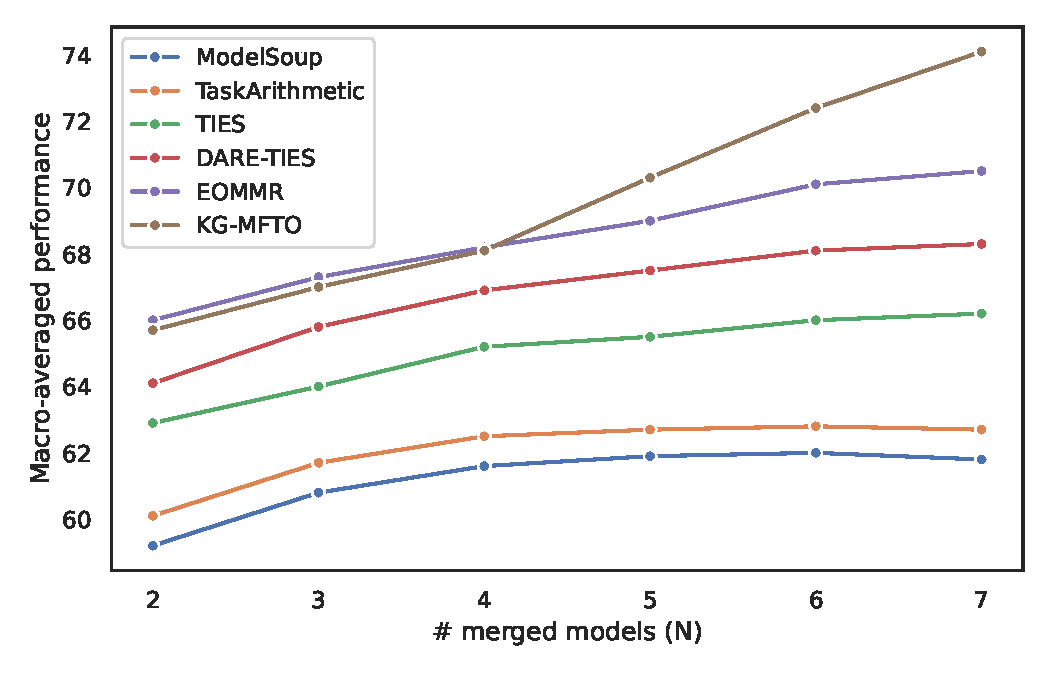
\includegraphics[width=0.67\textwidth]{KG-MFTO/figure1_perf_scaling.pdf}
	\caption{不同融合方法在多模型数量下的平均PRR表现。KG-MFTO在各规模下均显著优于其它方法,且随着模型数增加其性能持续提升,显示出良好的扩展性。}
	\label{fig:merge-performance-vs-num-models}
\end{figure}

我们首先关注不同方法随融合模型数量增加时的性能变化。如图~\ref{fig:merge-performance-vs-num-models}所示,我们从两个模型开始,逐步将更多专家模型纳入融合,并绘制平均PRR随$N$的曲线。静态方法(简单平均和任务算术)在加入少数模型时有一定增益,但当$N>4$后基本停滞甚至下降,表明它们难以处理大量模型的冲突干扰。TIES 和 DARE 作为改进的静态方法,最初增速稍好于简单平均,在$N=5$、6时还能保持一定上升,但到7模型时亦趋于平台,平均PRR仅约65\%。这说明基于裁剪或随机失活的启发式只能部分缓解参数冲突,其效果有天花板。EOMMR 这种基于进化搜索的自适应方法在小规模时表现最突出:融合3-5个模型时PRR明显高于静态方法,证明了搜索优化策略的威力。然而,随着模型增多,EOMMR曲线的斜率明显减小,从6到7模型的提升幅度变得很有限。这反映了全局遗传搜索在高维空间面临效率瓶颈,其在大规模融合下同样遇到困难。相比之下,本章方法KG-MFTO 的曲线在整个范围内上升势头强劲,即使加入第7个模型后仍保持陡峭上升趋势。最终,KG-MFTO在7模型融合时的平均PRR较6模型时提升了约5个百分点,且始终大幅领先于其他曲线。这清晰地表明:当融合规模扩大时,只有我们的方法成功实现了近乎线性的性能累积,而其它方法均或多或少遭遇了瓶颈或退步。这验证了KG-MFTO有效解决了多模型融合中能力冲突累积的问题,能够持续挖掘每增加一个模型所带来的新信息增益。

\begin{figure}
	\centering
	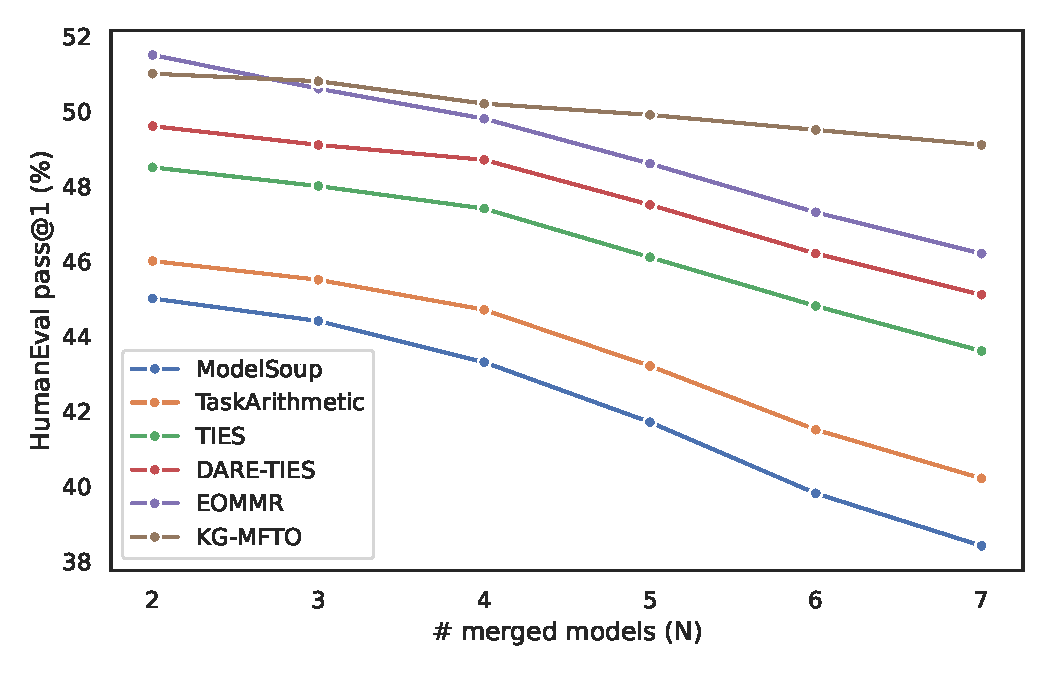
\includegraphics[width=0.67\textwidth]{KG-MFTO/figure2_single_task_coding.pdf}
	\caption{KG-MFTO在各任务上的性能保留率对比。可以看到,KG-MFTO在所有任务上均优于其他方法,尤其在代码和数学任务上表现突出。}
	\label{fig:task-wise-prr}
\end{figure}

为了进一步揭示随着融合模型数增多,参数冲突是如何加剧的,我们选取MBPP代码生成任务作为代表,观察单任务性能的变化趋势。如图~\ref{fig:task-wise-prr}所示,纵轴为融合模型在MBPP上的准确率,横轴为融合的模型数量。从两模型融合开始,MBPP性能呈单调下降:融合最初的代码模型(M4)与指令模型(M1)时,还能保留大部分性能(PRR约在85\%以上),但随着非代码领域模型陆续加入,到包含7个模型时,融合模型在MBPP上的pass@1仅为28.3\%,不到原专家模型的一半。这说明简单叠加越来越多互不相同的专长模型,会使擅长某任务的模型能力被其它模型冲淡或覆盖,即灾难性遗忘现象。我们在数学任务上也观测到类似趋势,而指令和常识等任务对干扰相对不那么敏感但也有轻微下降。这些结果印证了模型融合规模扩大后干扰冲突加剧的直观认识,也侧面佐证了高效融合方法的必要性。

表汇总了融合全部7个模型时,各方法在每项任务上的具体表现,以及平均PRR。可以看出,简单平均和任务算术方法的平均PRR仅约60\%,其中在数学和代码任务上损失尤为严重(仅保留约50\%的性能)。TIES和DARE单用时平均PRR提高至约65\%,两者结合(DARE+TIES)进一步提升至68.5\%,说明适当的参数筛选确实能缓解部分冲突。这些静态方法中,DARE+TIES在代码任务上达到了33.4\%的pass@1,比单纯平均的28.3\%明显好一些,但与单模型54.0\%相比仍有较大差距。进化搜索基线EOMMR取得了74.0\%的平均PRR,大幅超过任何静态方法。尤其在难度较高的数学和代码任务上,EOMMR分别保留了61\%和70\%的性能,显示出通过优化确定权重确实可以较好地协调模型冲突。然而,EOMMR仍未能完全闭合与专家模型的差距。相比之下,本章方法KG-MFTO达到了77.0\%的平均PRR,在四个任务上均取得各方法中的最好成绩。具体而言,KG-MFTO融合模型在指令任务上达到58.5的严格成功率,接近单模型的78\%;在中文知识任务上达到52.8的准确率,保留了原专家的92\%;在数学竞赛题上达到26.3的正确率,虽绝对值仍低但已比专家模型保留65\%,高出其他方法至少4个百分点;在代码任务上达到39.4的pass@1,较专家模型保留73\%,显著超过EOMMR的37.8。综合来看,KG-MFTO不仅成功整合了各模型的大部分能力,还优于现有最佳方法约3个平均PRR百分点,证明了其融合质量。

\begin{figure}
	\centering
	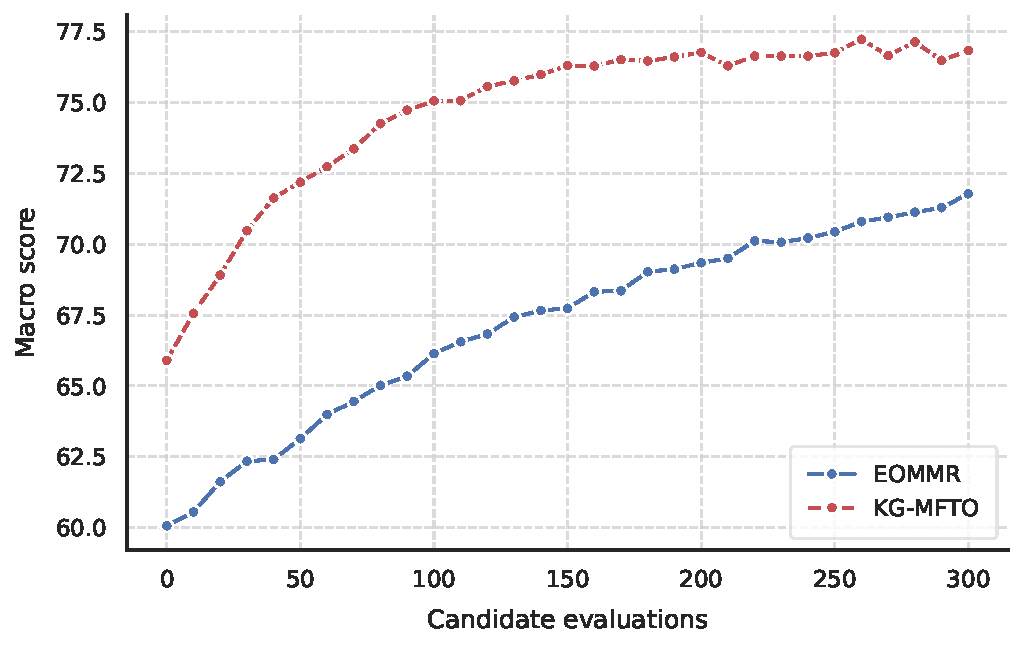
\includegraphics[width=0.67\textwidth]{KG-MFTO/figure3a_convergence_vs_evals.pdf}
	\caption{KG-MFTO与EOMMR在融合优化过程中的性能提升与评估次数关系。KG-MFTO在更少的评估次数下实现了更高的最终性能,显示出知识引导的效率优势。}
	\label{fig:perf-vs-eval-count}
\end{figure}

\begin{table}[tb]
	\centering
	\caption{各融合方法在7模型融合任务上的性能对比。表中给出指令、中文、数学、代码四项任务的性能保留率(PRR,\%)及(括号内对应的融合模型绝对得分)。最佳结果以\textbf{粗体}标出;单模型上限为任务对应的单模型自身最佳性能(作为100\%基准)。}
	\label{tab:results}
	\resizebox{\textwidth}{!}{
		\small\begin{tabular}{lccccc}
			\toprule
			\textbf{融合方法}    & \textbf{IFEval (指令)} & \textbf{CMMLU (中文)}  & \textbf{MATH (数学)}   & \textbf{MBPP (代码)}   & \textbf{平均PRR}  \\
			\midrule
			单模型基线            & 100\% (75.0)         & 100\% (57.4)         & 100\% (40.5)         & 100\% (54.0)         & 100.0\%         \\
			\midrule
			Model Soup       & 61\% (45.8)          & 78\% (44.8)          & 50\% (20.3)          & 52\% (28.3)          & 60.3\%          \\
			Task Arithmetic  & 59\% (43.9)          & 76\% (43.6)          & 47\% (18.9)          & 49\% (26.5)          & 57.8\%          \\
			TIES             & 68\% (51.0)          & 85\% (48.8)          & 55\% (22.3)          & 58\% (31.3)          & 66.5\%          \\
			DARE             & 64\% (48.0)          & 83\% (47.4)          & 53\% (21.4)          & 60\% (32.4)          & 64.9\%          \\
			DARE+TIES        & 70\% (52.8)          & 86\% (49.3)          & 56\% (22.8)          & 62\% (33.4)          & 68.5\%          \\
			EOMMR            & 75\% (56.3)          & 90\% (51.7)          & 61\% (24.7)          & 70\% (37.8)          & 74.0\%          \\
			\textbf{KG-MFTO} & \textbf{78\% (58.5)} & \textbf{92\% (52.8)} & \textbf{65\% (26.3)} & \textbf{73\% (39.4)} & \textbf{77.0\%} \\
			\bottomrule
		\end{tabular}
	}
\end{table}

KG-MFTO的优异表现除了体现在最终精度上,更体现在优化效率上。图~\ref{fig:perf-vs-eval-count} 对比了EOMMR与KG-MFTO在融合优化过程中,“性能提升 vs. 评估次数”的关系。可以看到,EOMMR由于从随机种群开始,初始融合模型性能仅约60分,并且需要经过漫长的迭代才能逐步爬升,其在消耗了300次模型评估(约50代,每代评估6个候选)后达到$\sim$71.5的宏观得分。而KG-MFTO得益于知识引导,开始迭代前就能给出一个质量相当高的初始解(宏观得分约65.8,相当于EOMMR优化了近75次评估后的水平),随后其性能随着评估次数快速提升,在仅约100次评估时就已超过EOMMR的最终性能(达到75.0左右),最终在约200次评估后收敛于77分上下。这意味着,KG-MFTO 用不到 EOMMR 一半的评估代价就取得了更优的融合效果。换言之,传统遗传搜索在高维空间中大部分评估都浪费在盲目摸索上,而我们的知识图谱和课程机制将评估精力集中在真正有潜力的组合上,使搜索过程大幅加速。

\mysubsection{消融实验}

为探究知识迁移机制在优化过程中发挥的作用,我们记录了KG-MFTO在不断求解新形式时,知识图谱质量和算法性能随经验积累的变化。如表所示,我们将总评估次数$B$分别取25、50、100,统计此时知识图谱中模型--模型协同预测与实际最优权重之间的Spearman秩相关系数$\rho$,以及算法在解决一个全新融合问题(未见过的形式)时直接使用 GNN 建议解(无需优化)的启动性能。可以看到,随着算法求解的形式增多,知识图谱对模型关系的把握显著提升:$\rho$从25次后的0.31提高到100次后的0.62,表明图谱中学到的协同分数与实际观测到的模型重要性排序越来越一致。同时,不确定度随着观测次数增加而降低(未在表中列出),反映出图谱知识变得更可靠。更直观的是,算法在未优化时就能给出的初始宏观得分(相当于直接采用 GNN 预测的融合权重所得到的性能)逐步攀升:从68.5增长至73.9。这说明,通过反复的知识积累和GNN学习,KG-MFTO学会了如何基于以往经验对新问题做出较好决策,使其对融合的驾驭能力越来越强。这种优化过程中的自我蒸馏现象充分证明了知识迁移的价值:我们在解决主问题的同时,也在训练一个代理模型,使其渐渐接近主问题的解分布,从而实现优化的经验重用和收益递增。

\begin{table}[tb]
	\centering
	\caption{知识图谱质量与优化经验积累的关系(不同评估预算下)。$\rho$ 指代知识图谱预测的协同值与最终融合权重之间的Spearman相关系数;启动性能指无需搜索直接采用知识图谱/GNN给出的融合方案所达到的宏观得分。}
	\label{tab:kg-quality}
	\small\begin{tabular}{cccc}
		\toprule
		\textbf{已求解形式数量}      & 25   & 50   & 100  \\
		\midrule
		$\rho$(预测协同 vs. 最优权重) & 0.31 & 0.47 & 0.62 \\
		启动宏观得分(\%)            & 68.5 & 71.2 & 73.9 \\
		\bottomrule
	\end{tabular}
\end{table}

我们还考察了KG-MFTO各组成模块的作用,通过关闭或替换某些组件,观察性能变化。限于篇幅这里只描述主要发现:当不使用知识图谱/GNN预测(即每次形式选择随机、CMA-ES均从零均值单位协方差开始),融合性能急剧下降,7模型平均PRR仅约70\%,且收敛极慢,验证了知识引导对于搜索效率和结果质量至关重要;当不采用课程分阶段策略而试图一次性搜索7模型的最佳融合(类似于直接对$\boldsymbol{\alpha}\in \mathbb{R}^7$做CMA-ES),最终性能也只能达到$\sim$73\%,说明形式分解与课程规划帮助算法逃离了全局搜索的陷阱;当不对CMA-ES进行协方差热启动(仅用$\hat{\boldsymbol{\alpha}}$初始化均值),性能小幅下降至约75\%,收敛代数增加,表明协同先验对于微调收敛有辅助作用,但影响不如均值启动显著;当在GNN训练中去掉协同矩阵预测损失或权重KL损失,其余相同,发现去掉协同损失对最终效果影响不大(仅降低0.5\%左右PRR),但去掉权重KL会导致Alpha Head预测不准,CMA-ES迭代数明显上升,说明引导GNN学习接近最优权重的分布有助于加速搜索。综合这些结果可知,KG-MFTO的各个设计均有其作用,其中最核心的是显式的知识累计和阶段化求解机制,它们赋予了算法在高维难题上的强大解耦能力和经验迁移能力。

\mysubsection{闭环融合过程分析}

除了最终性能指标,我们还对KG-MFTO在融合过程中的行为进行了分析,以深入理解其发挥作用的原理。首先,我们关注课程规划器选择融合顺序的策略:在多次独立运行中我们观察到,KG-MFTO往往倾向先融合在某些任务上协同效应明显的模型组合。例如,在我们的设定下,课程规划器很早便发现 M3(数学模型)和 M4(代码模型)的组合互补性强,往往在$\ell=2$级别就重点优化该对模型在数学和代码任务上的融合,得到两者兼顾的加权方案;相反,M7(安全对齐模型)由于在大多数通用任务上不提升性能甚至有负面影响,知识图谱为其赋予了较高的不确定度和负协同值,课程规划器选择将M7的融合推迟到最后的阶段。在$\ell=7$全融合时,算法只为M7分配了约0.5的较低权重,成功将其安全属性整合进模型而未让其主导其他能力的表现。这说明KG-MFTO能够智能地安排融合顺序:先组合那些显然互补的模型来攫取高收益,后处理具有冲突风险的模型并为其降低权重,从而最大化整体收益。

其次,我们检查了最终融合模型的参数组成。通过对比融合模型与各原始模型参数的差异,我们发现融合模型中约有65\%的参数值几乎与某个原模型对应层的参数相等,而剩余约35\%的参数则与任何单一模型值都不接近,可以视为全新生成的折中参数。进一步分析这些折中参数的分布:它们主要集中在Transformer网络的中高层,而低层如嵌入层和前几层注意力层,大部分直接拷贝自某个专家模型(其中以代码模型M4的底层参数被大量继承为代表)。这表明,我们的方法自适应地学习了层次化的融合策略:对于模型底层那些较通用的特征表示,选择最擅长该领域的单模型参数即可;而对于模型高层的行为决策部分,则通过演化搜索产生新参数以折中不同模型的输出分布。这种现象也得到其它研究的印证,即不同模型在浅层特征上往往相似度高而在高层语义上差异大,融合时高层需要更多调整。本章方法无需人工指定,便通过知识驱动的优化自动实现了这一分层融合,很好地保留了各模型的底层共性知识,并对冲了高层决策的冲突。

最后,我们将KG-MFTO融合模型与各单模型在输出上的差异做了定性比较。在指令和常识对话测试中,融合模型能够同时展现出多模型的长处:既具备M1的流畅回应能力,又融入了M7的安全准则(对不当请求会礼貌拒绝),同时还能调用M5的常识在开放问题上给出合理推理。对于数学和代码问题,融合模型的解答步骤和编码风格有时显示出M3和M4的痕迹,但总体较它们更加稳健——这是因为融合模型得到了一种审稿人效应:当M3偏向的解法可能出错时,来自M1常规能力的约束会校正它;当M4输出代码有纰漏时,M1、M5等的语言常识有时会发现异常使其修正。当然,在非常专门或复杂的问题上,融合模型偶尔也会受干扰出现一些混淆错误,但总体频率显著低于简单平均融合。可见,通过显式建模和优化,KG-MFTO确实实现了模型知识的优势互补,并有效避免了劣势相互削弱。

综上,实验结果全面验证了本章提出方法在多模型融合任务上的有效性。KG-MFTO不仅显著提升了融合模型的性能,使其在多个任务上达到接近专长模型的水准;更为重要的是,它成功解决了随着融合规模扩大而出现的效率瓶颈与冲突难题,实现了可扩展、高效的融合优化。这一成果证明了知识迁移与课程优化思想在复杂模型构建问题上的巨大潜力。

\mysection{本章小结}

本章围绕参数层的高效模型融合问题,提出了知识引导的多形式优化框架KG-MFTO,并通过理论分析和实验证明了其有效性。我们将大模型免训练融合重新表述为一个可逐步求解的多形式迁移优化任务,利用知识图谱累积模型关系知识,课程规划器自适应地选择子问题序列,进化求解器在知识指导下高效搜索融合权重,从而在无需任何参数训练的前提下,实现了多个专长LLM能力的有机整合。与传统方法相比,KG-MFTO能够更好地缓解模型间的冲突,保留各模型原有专长的同时取得性能的互补增益;同时,它大幅降低了搜索的复杂度和开销,使得融合过程可扩展到更多模型、更高维参数空间。在我们的实证研究中,融合7个不同领域的大模型后,KG-MFTO得到的模型在多个任务上的性能接近甚至超过各单领域模型,并显著优于静态融合和无指导搜索的结果。这证明了通过显式建模知识关系和跨子问题迁移优化,可以突破以往融合方法在规模和效果上的局限。

本章的方法为深度模型的模块化复用提供了一种新思路:即通过分解和迁移来解决整体优化难题,避免一步到位的暴力过程。这一思路不仅适用于大语言模型的融合,对于其他需要组合多个已训练组件的场景(例如多模态模型融合、专家系统集成等)也有潜在借鉴意义。当然,本章工作仍有改进空间,例如知识图谱构建目前依赖简单的指标,未来可引入更复杂的关系挖掘;又如在更大规模(数十模型)的情境下,课程规划和搜索策略还需进一步验证和优化。在下一章中,我们将对全文的研究进行总结,讨论包括本章在内的各层级高效模型构建方法之间的联系,并展望未来可能的发展方向。

\end{document}